% Made up for the tikra benchmark.
\usetikzlibrary{datavisualization.formats.functions}
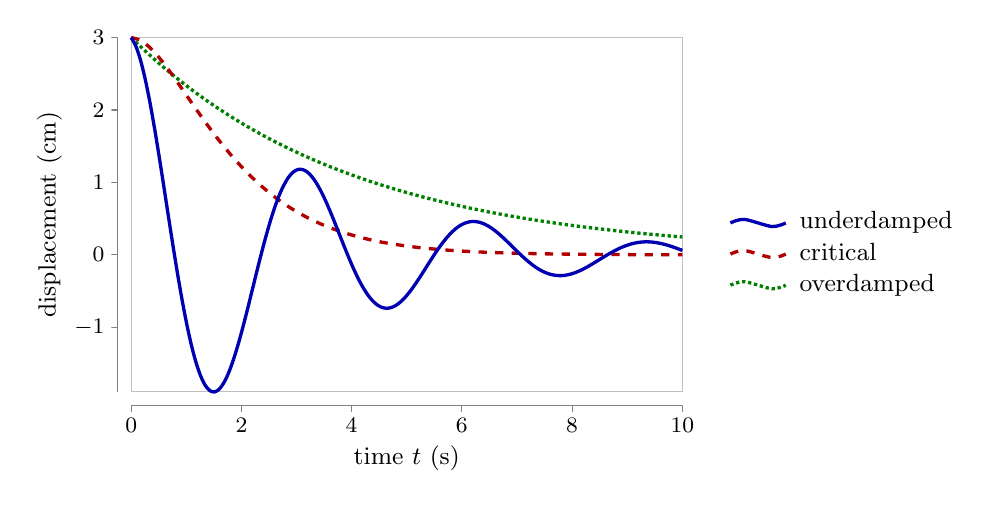
\begin{tikzpicture}
  \datavisualization [scientific axes=clean,
      x axis={label=time $t$ (s), length=7cm},
      y axis={label=displacement (cm), length=4.5cm},
      visualize as smooth line/.list={under, critical, over},
      under={style={blue!70!black, very thick}, label in legend={text=underdamped}},
      critical={style={red!70!black, very thick, dashed}, label in legend={text=critical}},
      over={style={green!50!black, very thick, densely dotted}, label in legend={text=overdamped}}]
    data [set=under, format=function] {
      var x : interval [0:10] samples 120;
      func y = 3*exp(-0.3*\value x)*cos(2*\value x r);
    }
    data [set=critical, format=function] {
      var x : interval [0:10] samples 60;
      func y = 3*(1+\value x)*exp(-\value x);
    }
    data [set=over, format=function] {
      var x : interval [0:10] samples 60;
      func y = 3*exp(-0.25*\value x);
    };
\end{tikzpicture}
